\section{Results}
The model was applied to the IEEE 14-bus network and a single loading scenario, shown in Fig.~\ref{fig:base}. The contingency list contained all
branches, that is, $\mathcal{C}= \mathcal{E}$, and all contingencies were assumed to be equally likely. It was modeled in Julia and solved by Gurobi 11 on an Apple M3. The computation time was 1.8 seconds, which in Gurobi's metric corresponds to 3.26 work units.

Figs.~\ref{fig:base}-\ref{fig:intermediate} each consist of two panels. The pre-contingency scenario is shown on the left. 
Buses represented as circles are
generating, while those represented as squares are consuming. Their sizes follow
the absolute value of their injections, and net consumption (in MW) is given. Branches are color coded as black (opened by the OTS algorithm) or green (closed), where arrows and numbers indicate the flow (in MW). 

The security analysis is shown on the right of each figure. The title of each subfigure
is the name of the branch that tripped. It is in bold style when a part of the
grid is de-energized and the load lost is in brackets. 
In the security analysis figures, the lines opened
by the OTS algorithm are removed, dashed black lines are those the contingency one, and solid black lines those that are in a de-energized area. The already opened lines are removed and overloaded lines are shown in red.

\begin{figure}[h]
    \begin{subfigure}
        [t]{.43\linewidth}
        \includegraphics[width=\linewidth]{images/case_base.pdf}
        \caption{base case}
        \label{fig:case base}
    \end{subfigure}\hfill
    \begin{subfigure}
        [t]{.48\linewidth}
        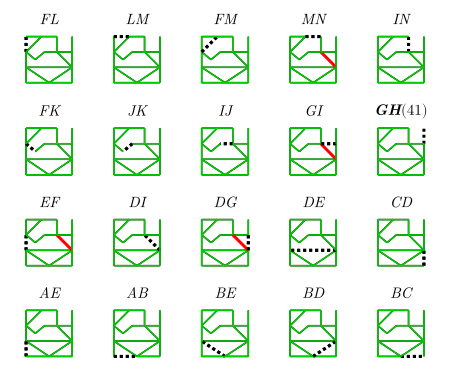
\includegraphics[width=\linewidth]{images/grid_base.pdf}
        \caption{security analysis}
        \label{fig:grid base}
    \end{subfigure}
    \caption{Base without OTS: There is no overflow in the base case. The
    security analysis reveals that numerous trippings raise an overload on $ID$.}
    \label{fig:base}
\end{figure}

The base case is shown in Figure \ref{fig:case base}. There is no overloading; therefore,
if branches are to be open, it is only to cope with overloads in N-1. The source
vertex corresponds to the bus $A$, which holds the largest generator. Figure \ref{fig:grid
base} shows the results of the security analysis where 4 of 20 trippings end with
the overload of the branch $DI$. As $GH$ forms an antenna, its tripping results in
the loss of the bus $H$.

\begin{figure}
    \begin{subfigure}
        [t]{.43\linewidth}
        \includegraphics[width=\linewidth]{images/case_ots.pdf}
        \caption{base case}
        \label{fig:case ots}
    \end{subfigure}\hfill
    \begin{subfigure}
        [t]{.48\linewidth}
        \includegraphics[width=\linewidth]{images/grid_ots.pdf}
        \caption{security analysis}
        \label{fig:grid ots}
    \end{subfigure}
    \caption{Base case with OTS. 
    The main connected component is defined as the one containing A.}
    \label{fig:ots}
\end{figure}

Figure \ref{fig:case ots} shows the situation with the branch opening proposed
by our algorithm. As expected, there is no overloading anymore as shown by the
security analysis in Figure \ref{fig:grid ots}, but this comes at the cost of loss of
buses for for 8 of 14 contingencies. Now, $DI$ only holds an antenna with the load
of the buses $I$ and $J$ and its load will never exceed the sum of both consumptions.
However, to isolate this antenna, $IG$ is opened, which grows the previously existing
antenna with $G$ and $H$. In addition, $IN$ and $IJ$ are opened, creating a
peninsula held on branch $EF$ with the buses $F$, $K$, $L$, $M$ and $N$.

\begin{figure}[h]
    \begin{subfigure}
        [t]{.43\linewidth}
        \includegraphics[width=\linewidth]{images/case_intermediate.pdf}
        \caption{base case}
        \label{fig:case intermediate}
    \end{subfigure}\hfill
    \begin{subfigure}
        [t]{.48\linewidth}
        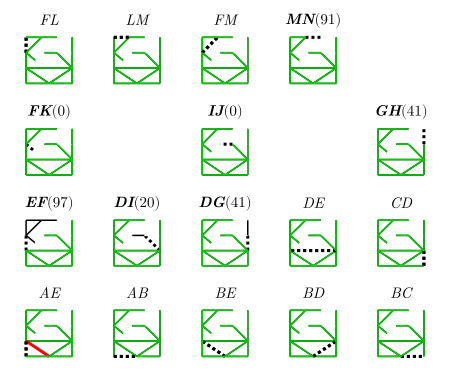
\includegraphics[width=\linewidth]{images/grid_intermediate.pdf}
        \caption{security analysis}
        \label{fig:grid intermediate}
    \end{subfigure}
    \caption{Intermediate case that the operator would needed to step into. The branch
    openings in the northern area solve the constraint on branch $DI$, but
    raises a constraint on the branch $BE$. }
    \label{fig:intermediate}
\end{figure}

That scenario also reveals the preventive-openings-cascade phenomenon. In fact, in the
base case, only the branch $DI$ is at risk of being overloaded and the opening of
$JK$, $IN$ and $GI$ may appear at first sufficient. Figure
\ref{fig:intermediate} shows the intermediate state if the operator only focuses
on the initial constraint. None of the trippings in the northern area leads to overloads.
But that reconfiguration also affected the distribution of the flows in the
southern part, which raises a new constraint. Now, the tripping of $AE$, which
was previously sound, ends with the overloading of the branch $BE$. Thus, resolving
the constraint in the northern area weakens the southern one, and consequently a
reconfiguration becomes also necessary in that area: the opening of the branches
$BE$, and $CD$ and now, $BC$ becomes an antenna.

This rationale is similar to what would have been necessary for an operator facing
the same situation. Sometimes back and forth steps are necessary. This kind of iterative
approach is time consuming even for such a simple case, and the operator would
settle for a solution that respects the security rules, even if it may be far from
optimal. Thanks to the optimization technique, all the constraints are incorporated
into one single problem and then solved at once. Moreover, by taking into account
the probability associated with the tripping of each individual line, as well as
the subsequent loss, a solution can be found that completely avoids the exposure to the unknown risks associated with overloading and minimizes the risk related to de-energized buses. 
%reduces the overall risk exposure to the risk of loss.
The performance is summarized in Table~\ref{tab1}.


\begin{table}[htbp]
\caption{Result summary}
\begin{center}
\begin{tabular}{|c|c|c|c|}
\hline
\textbf{}&\multicolumn{3}{|c|}{\textbf{Scenario}} \\
\cline{2-4} 
\textbf{metric} & \textbf{\textit{base}}& \textbf{\textit{intermediate}}& \textbf{\textit{optimized}} \\
\hline
preventive branch openings & 0 & 3 & 5 \\
    contingencies with overloads & 4 & 1 & 0\\
     contingencies with de-energized buses & n/a$^{\mathrm{a}}$ & n/a$^{\mathrm{a}}$ & 8 \\
     average demand loss, per contingency & n/a$^{\mathrm{a}}$ & n/a$^{\mathrm{a}}$ & 6.7\% \\
\hline
\multicolumn{4}{l}{$^{\mathrm{a}}$due to overloads, consequences are unknown.}
\end{tabular}
\label{tab1}
\end{center}
\end{table}
